\documentclass{standalone}
\usepackage{tikz}
\usetikzlibrary{calc}
\begin{document}
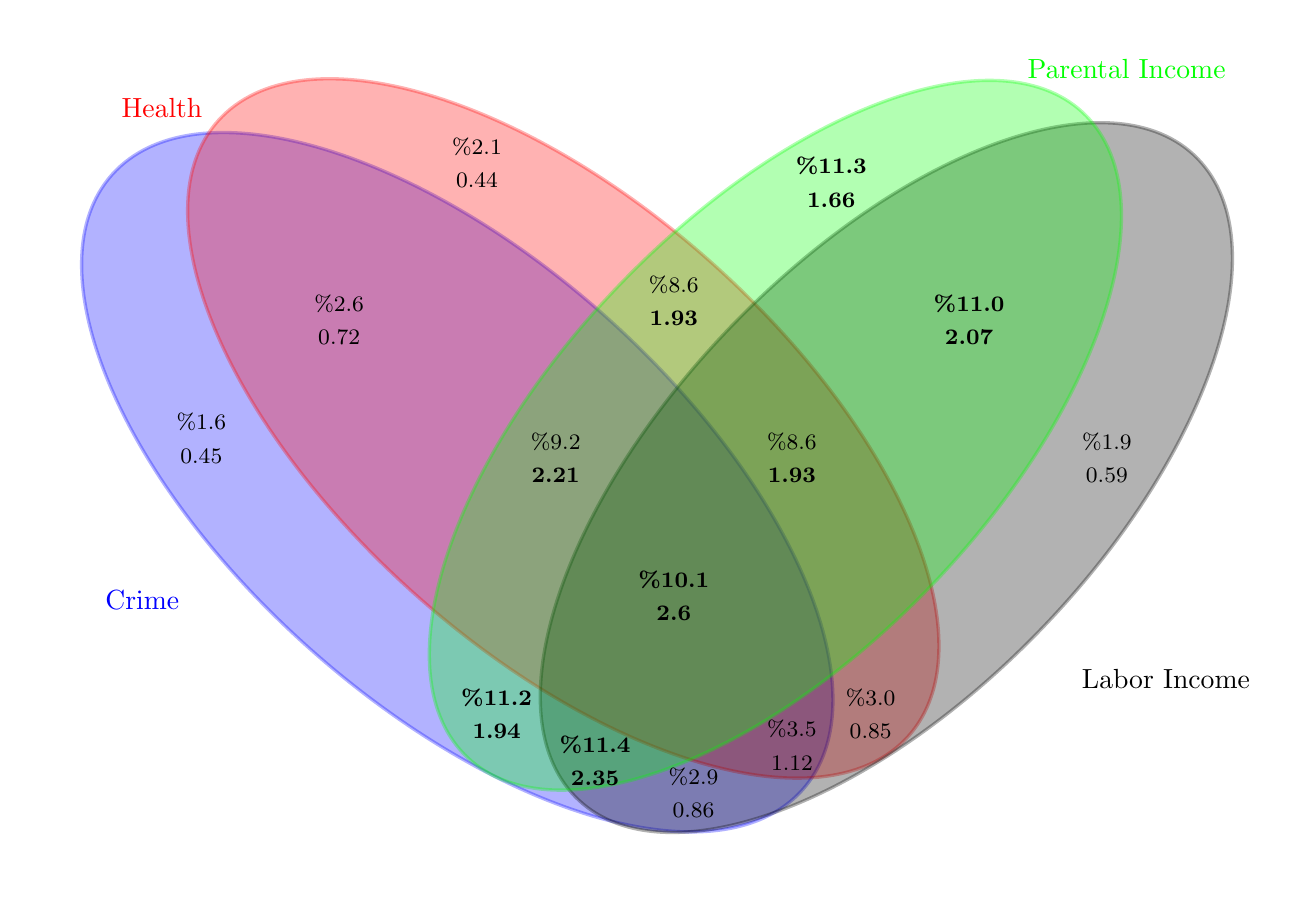
\begin{tikzpicture}

\begin{scope}[shift={(-2,0)},x={(2,2)},y={($(-2,0)!1!60:(2,2)$)}]
  \draw[blue, very thick, fill=blue, opacity=.3] (.5,0) ellipse (1 and .5);
\end{scope}
\begin{scope}[shift={(-2,0)},x={(2,2)},y={($(-2,0)!1!60:(2,2)$)}]
  \draw[red, very thick, fill=red, opacity=.3] (1,-.04) ellipse (1 and .5);
\end{scope}

\begin{scope}[shift={(2,0)},x={(-2,-2)},y={($(2,0)!1!60:(-2,-2)$)}]
  \draw[black, very thick, fill=black, opacity=.3] (-.9,-0.125) ellipse (2 and .35);
\end{scope}
\begin{scope}[shift={(2,0)},x={(-2,-2)},y={($(2,0)!1!60:(-2,-2)$)}]
  \draw[green, very thick, fill=green, opacity=.3] (-.65,.05) ellipse (2 and .35);
\end{scope}

\draw (-4.25,2) node[align=center, below][align=center, below] {\footnotesize \%1.6 \\ \footnotesize  0.45}; 		%A
\draw (-0.75,5.5) node[align=center, below] {\footnotesize \%2.1 \\ \footnotesize  0.44}; 						%B
\draw (3.75,5.25) node[align=center, below] {\footnotesize \textbf{\%11.3} \\ \footnotesize  \textbf{1.66}}; 				%C
\draw (7.25, 1.75) node[align=center, below] {\footnotesize \%1.9 \\  \footnotesize 0.59}; 						%D
\draw (-2.5,3.5) node[align=center, below] {\footnotesize \%2.6 \\ \footnotesize  0.72}; 						%AB
\draw (-.5,-1.5) node[align=center, below] {\footnotesize \textbf{\%11.2} \\ \footnotesize  \textbf{1.94}}; 				%AC
\draw (2,-2.5) node[align=center, below] {\footnotesize \%2.9 \\ \footnotesize  0.86}; 						%AD
\draw (1.75,3.75) node[align=center, below] {\footnotesize \%8.6 \\ \footnotesize  \textbf{1.93}}; 					%BC
\draw (4.25,-1.5) node[align=center, below] {\footnotesize \%3.0 \\ \footnotesize  0.85}; 						%BD
\draw (5.5,3.5) node[align=center, below] {\footnotesize \textbf{\%11.0} \\ \footnotesize  \textbf{2.07}}; 			%CD
\draw (0.25, 1.75) node[align=center, below] {\footnotesize \%9.2 \\ \footnotesize  \textbf{2.21}}; 					%ABC
\draw (3.25,-1.9) node[align=center, below] {\footnotesize \%3.5 \\ \footnotesize  1.12}; 						%ABD
\draw (0.75,-2.1) node[align=center, below] {\footnotesize \textbf{\%11.4} \\ \footnotesize  \textbf{2.35}}; 			%ACD
\draw (3.25, 1.75) node[align=center, below] {\footnotesize \%8.6 \\ \footnotesize \textbf{1.93}}; 					%BCD
\draw (1.75,0) node[align=center, below] {\footnotesize \textbf{\%10.1} \\ \footnotesize \textbf{2.6}}; 													%ABCD


\draw [blue] (-5,-.25) node[align=center, below] {Crime};
\draw [red] (-4.75,6) node[align=center, below] {Health};

\draw [black] (8,-1.25) node[align=center, below] {Labor Income};
\draw [green] (7.5,6.5) node[align=center, below] {Parental Income};



\end{tikzpicture}
\end{document}


